\multiproblem{1}{
  Consider a rod of known length $l$ and mass $m$ resting on
  three supports, as shown.\\
  \begin{minipage}{0.6\textwidth}
    \vspace{0.1in}
    \begin{enumerate}
      \item Draw a free-body diagram for the rod. Suppose we know that
        $N_{3}=4\newtons$. Use the external force balance and moment balance
        about $A$ to find the reaction forces $N_{1}$ and $N_{2}$.
      \item Consider the case where all reaction forces at the supports are
        unknown. Find the external force balance and the moment balance about
        points $A$ and $B$. Write the system in the form ${\bf A x}={\bf b}$,
        where ${\bf x}=(N_{1},N_{2},N_{3})^{T}$, ${\bf A}$ is a $3\times 3$
        matrix of known values and ${\bf b}$ is a $3 \times 1$ vector of known
        values.
      \item Construct the augmented matrix $(\mathbf{A}|\mathbf{b})$ and use
        this to solve for ${\bf x}$ and find the set of all possible values for
        the reaction forces $N_{1}$, $N_{2}$ and $N_{3}$. Is the system
        statically indeterminate?
      \item From the resting constraint $N_{i}>0$. Use this to find the minimum
        and maximum values of each of the reaction forces.
    \end{enumerate}
  \end{minipage}
  \begin{minipage}{0.3\textwidth}
    \begin{center}
      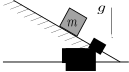
\includegraphics[scale=1.5]{fig_1.pdf}
    \end{center}
  \end{minipage}
}

\multiproblem{2}{
  A body is acted upon by three forces at the points $A$, $B$, and $C$ which
  have position vectors $(1, 2)\metres$, $(5, 1)\metres$ and $(4, 3)\metres$
  respectively. The force acting at $A$ is $\mathbf{F}_A = (2, 7)\newtons$
  \begin{enumerate}
    \item Draw a good diagram of this body and the forces acting on it. The
      shape of the body is irrelevant for your answers to this question but
      feel free to draw it as the triangle $ABC$.
    \item Suppose that the force $\mathbf{F}_B=\mathbf{0}$. What would
      $\mathbf{F}_C=(F_{C1},F_{C2})$ need to be for force and moment balance
      to hold?
    \item Suppose instead that the force $\mathbf{F}_B=(F_B,0)$ for what
      values of $F_B$, $F_{C1}$ and $F_{C2}$ would there be equilibrium?
    \item Now suppose that we know nothing about either of $\mathbf{F}_B$ and
      $\mathbf{F}_C$. Find the set of all possible combinations of
      $\mathbf{F}_B$ and $\mathbf{F}_C$ for which equilibrium is possible.
    \item Use your understanding of linear systems with different numbers of
      equations and unknowns to explain why we get the three different
      situations seen in the previous parts.
  \end{enumerate}
}

\multiproblem{3}{
  A uniform rod of mass $m$ and length $L$ is connected by a pin support to
  the wall at one end and suspended from the wall by a light inextensible
  string that is attached to the other end of the rod at a known angle
  $\theta$, as shown.\\
  \begin{minipage}{0.6\textwidth}
    \begin{enumerate}
      \item Draw a free-body diagram for the rod. Assuming the system is in
        static equilibrium, find the tension in the string.
      \item Now find the contact force at the pin support. What angle does it
        make to the horizontal?
      \item Show that the lines of action of all three forces intersect at a
        single point. Argue that this should always happen for a body acted
        upon by three forces.
    \end{enumerate}
  \end{minipage}
  \begin{minipage}{0.3\textwidth}
    \begin{center}
      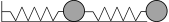
\includegraphics[scale=1.8]{fig_3.pdf}
    \end{center}
  \end{minipage}
}

\multiproblem{4}{
  A uniform rod of mass $m$ and length $L$ learns against a wall. A mass
  $m_{1}$ is attached a distance $x$ from point $A$.
  \begin{center}
    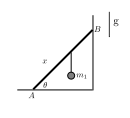
\includegraphics[scale=1.8]{fig_4.pdf}
  \end{center}
  \begin{enumerate}
    \item Let $x=2l/3$. Draw free-body diagrams for both bodies. Assume that
      friction acts at $A$, with known coefficient of friction $\mu_{A}$, but
      not at $B$. What are the three reaction forces? For what values of
      $\theta$ is static equilibrium possible?
    \item Assume friction acts at $B$ but not $A$? Now for which values of
      $\theta$ is static equilibrium possible?
    \item Now assume that friction acts at both $A$ and $B$. Find the set of
      solutions for the contact forces. Is the system statically determinate?
      Assume it now is about to slip at $B$. What are the contact forces now?
    \item Assume the rod is about to slip at $A$ and $B$ simultaneously. Can
      you find the contact forces? Allowing $m_{1}$ to be moved, where should
      it be placed to ensure static equilibrium?
  \end{enumerate}
}

\multiproblem{5}{
  Two rods are resting between two smooth walls and a smooth floor. We use a
  coordinate system that places the orign at the lower left corner of the
  room. The first rod has length $10\metres$ and mass $2m$ and rests with one
  end in the corner of the room at $(0,0)\metres$ and the other end against
  the opposite wall at $(8,6)\metres$. The second rod has length $5\metres$
  and mass $m$ and rests between the first rod and the left-hand wall from
  $(4,3)\metres$ to $(0,6)\metres$ as shown.\\
  \begin{minipage}{0.6\textwidth}
    \vspace{0.1in}
    \begin{enumerate}
      \item Assume that there is no friction between the rods and the
        walls/floor. For equilibrium find the values of all of the normal
        reaction forces between the rod/wall, rod/floor and rod/rod contacts
        and the value of the friction force between the two rods.
      \item What is the minimum value of the friction coefficient $\mu$ between
        the two rods to ensure that equilibrium is possible?
      \item Suppose we move the end of the upper rod so that it rests on a
        different part of the lower rod (but still has the same length).  Given
        a particular value for the friction coefficient $\mu$ what possible
        positions can the rod-rod contact point have for equilibrium to occur?
        Are there some positions that won't work for any value of $\mu$?
    \end{enumerate}
  \end{minipage}
  \begin{minipage}{0.3\textwidth}
    \begin{center}
      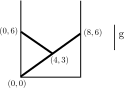
\includegraphics[scale=1.8]{fig_5.pdf}
    \end{center}
  \end{minipage}
}
